%! Author = angela
%! Date = 24/01/24
% !TeX root = ../thesis-main.tex

\chapter{Contributions}
\label{ch:contributions}
In this chapter, will be presented the main contributions of this thesis.

\section{Collektive}
\label{sec:collektive}

\emph{Collektive} is a framework designed to simplify the definition of \ac{ac} systems.

The main objective of this technology is to facilitate the development of aggregate programs that can be executed on a
variety of computing systems, such as mobile and wearable devices, computers, and the cloud.
This allows for interoperability and communication between these systems, despite their different nature.

To achieve this, \emph{Collektive} uses the \ac{fc} model to provide a straightforward and intuitive method for defining
an aggregate program, without the need for low-level coding.

In addition, \emph{Collektive} has been developed to be multiplatform, so it can be executed on different systems thanks
to the use of \emph{Kotlin Multiplatform}.

As for the feature solution of alignment for the correct functioning of aggregate programming,
it has been developed a compiler plugin with the purpose of annotating the functions that are aligned;
those paths will be used for the actual alignment of the nodes.

\section{DSL}
\label{sec:dsl}

In this thesis, the original implementation of the \ac{dsl} of \emph{Collektive} will be modified to allow the use of \xc{}
and to improve its performance.

\subsection{Architecture}
\label{subsec:architecture}

\subsection{XC in Collektive}
\label{subsec:exchange-in-collektive}

Thanks to the design of \xc{}, it is possible to implement the methods proposed by \emph{field calculus}
(~\ref{par:syntax-of-field-calculus}) in terms of \emph{exchange} (~\ref{par:communication-in-xc}).

The syntax of \emph{XC} allows for sending messages to specific nodes, enabling the implementation of \emph{field calculus}
operations through message exchange.

The \emph{exchange} communication is based on \emph{anisotropic} communications, meaning that it has not the same properties
or characteristics in all directions (\Cref{fig:anisotropic}); therefore, messages have custom values sent to different neighbours.

\begin{figure}[h!]
    \centering
    \includegraphics[width=0.2\textwidth]{figures/anisotropic}
    \caption{Anisotropic communication.}
    \label{fig:anisotropic}
\end{figure}

This concept can be extended to the \emph{share} function of field calculus, with the difference that the
operation of \emph{share} is based on \emph{isotropic} communication, meaning that properties are uniform in all directions
(\Cref{fig:isotropic}); therefore, messages have the same value sent to all neighbours.

\begin{figure}[h!]
    \centering
    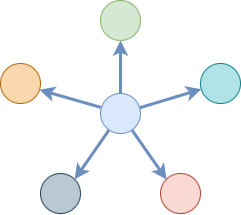
\includegraphics[width=0.2\textwidth]{figures/isotropic}
    \caption{Isotropic communication.}
    \label{fig:isotropic}
\end{figure}

\paragraph{Syntax}
%il dsl è stato modificato in maniera tale da sfruttare exchange per la costruzione degli altri costrutti quali share e neighbouring
%solamente il costrutto rep non viene implementato in termini di exchange, in quanto essendo una funzione che permette di iterare su
%se stessi, non vogliamo che i vicini ricevano messaggi di alcun genere, questo anche per questioni di sicurezza e privacy

All the \ac{dsl} has been modified to use \emph{exchange} for the implementation of the other constructs such as \texttt{share}
and \texttt{nbr}, which here is called \texttt{neighboring}.
Only the \emph{rep} construct has not been implemented in terms of \emph{exchange}, as it is a function

\subsection{Messages}
\label{subsec:messages}
%message modelling (in scafi there is an action that computes the messages and then creates a reaction that
%sends the message) we do it in a different way

\subsection{Syntax}
\label{subsec:syntax}
%code
%rep non serve farla con xc perche non vogliamo che gli altri nodi ricevano il messaggio, cose che non gli interessano

\section{Plugin Extensions}
\label{sec:plugin-extensions}

\paragraph{Alignment}
%how

\section{Incarnation}
\label{sec:incarnation}
%how, why

%gradle task

\section{Technologies}
\label{sec:technologies}
%multiplatform

\section{Implementation}
\label{sec:implementation}
%diagrams



